\chapter{Fundamentos}
\label{cap:fundamentos}

Neste capítulo, apresentamos definições fundamentais sobre redes bayesianas, redes soma-produto e diagramas de decisão algébrica, que o leitor deve conhecer para compreender o trabalho.

Assumimos que o leitor conhece noções básicas de conjuntos, grafos e que está familiarizado com teoria de probabilidades discretas \cite{Koller2009}.

\section{Redes bayesianas}

Redes bayesianas são modelos probabilísticos baseados em grafo que representam distribuições de probabilidade conjunta e são usados para raciocinar em situações com incerteza. Formalmente, ela é definida \cite{Nie2014} da seguinte forma:

\begin{definition}[rede bayesiana]
  Seja $N = \{ 1, \cdots, n \}$ e seja $X = \{X_i : i \in N\}$ um conjunto de variáveis aleatórias $X_i$ tomando valores em conjuntos finitos $\mathcal{X}_i$. Uma \textbf{rede bayesiana} é uma tripla $(X, G, \theta)$, onde $G = (V, E)$ é um DAG (que chamamos de \textbf{estrutura} da rede bayesiana) cujos vértices correspondem a variáveis em $X$ e $\theta = \{\theta_i(x_i, x_{\pi_i})\}$ é um conjunto de parâmetros numéricos especificando valores de probabilidade condicional $\theta_i(x_i, x_{\pi_i}) = P(x_i | x_{\pi_i})$ para todo vértice $i \in V$, valor $x_i \in X_i$ e atribuição $x_{\pi_i}$ para os pais $\pi_i$ de $X_i$ (em $G$).
\end{definition}

Um exemplo de rede bayesiana é mostrado na figura \ref{fig:bayes}. Intuitivamente, as arestas codificam dependências entre as variáveis.

\begin{figure}
  \centering
  \scalebox{0.7}{
    \begin{tikzpicture}
        [scale=.5,auto=left,every node/.style={draw, ellipse, inner sep = 3pt, minimum width = 0.72cm, align = center}]

        \node[fill=gray!30] (or) at (1,9) {$S$};
        \node[fill=gray!30] (al) at (7,9) {$A$};
        \node[fill=gray!30] (no) at (2,5) {$N$};
        \node[fill=gray!30] (me) at (10,5) {$M$};
        \node[fill=gray!30] (ca) at (0,1) {$C$};

        \path (or) edge[-triangle 60] (no)
          (al) edge[-triangle 60] (no)
          (al) edge[-triangle 60] (me)
          (no) edge[-triangle 60] (ca);

        \node[draw=none,inner sep = 0pt,above=of or]
        {
          \begin{tabular}{|c|c|} \hline
            $o_0$ & $o_1$ \\ \hline
            0,5 & 0,5 \\ \hline
          \end{tabular}
        };

        \node[draw=none,inner sep = 0pt,above=of al]
        {
          \begin{tabular}{|c|c|} \hline
            $a_0$ & $a_1$ \\ \hline
            0,5 & 0,5 \\ \hline
          \end{tabular}
        };

        \node[draw=none,inner sep = 0pt,below=of me]
        {
          \begin{tabular}{|c|c|c|} \hline
                  & $m_0$ & $m_1$ \\ \hline
            $a_0$ & 0,8 & 0,2 \\ \hline
            $a_1$ & 0,2 & 0,8 \\ \hline
          \end{tabular}
        };

        \node[draw=none,inner sep = 0pt,left=of no]
        {
          \begin{tabular}{|c|c|c|} \hline
                  & $n_0$ & $n_1$ \\ \hline
            $a_0,o_0$ & 0,9 & 0,1 \\ \hline
            $a_0,o_1$ & 0,7 & 0,3 \\ \hline
            $a_1,o_0$ & 0,5 & 0,5 \\ \hline
            $a_1,o_1$ & 0,1 & 0,9 \\ \hline
          \end{tabular}
        };

        \node[draw=none,inner sep = 0pt,below=of ca]
        {
          \begin{tabular}{|c|c|c|} \hline
                  & $c_0$ & $c_1$ \\ \hline
            $n_0$ & 0,9 & 0,1 \\ \hline
            $n_1$ & 0,1 & 0,9 \\ \hline
          \end{tabular}
        };
    \end{tikzpicture}
  }

  \caption{Exemplo de rede bayesiana com distribuições de probabilidade condicional.}
  \label{fig:bayes}
\end{figure}

Redes bayesianas são geralmente usadas para computar a probabilidade de alguma hipótese quando alguma evidência é observada. Por exemplo, uma rede bayesiana pode representar as relações de probabilidade entre doenças e sintomas. Observados alguns sintomas, a rede pode ser usada para computar a probabilidade da presença das doenças. Chamamos esse processo de \textbf{inferência}.

\section{Redes soma-produto}

Uma \textbf{rede soma-produto} \cite{Poon2012} é um grafo acíclico dirigido enraizado no qual as folhas são indicadores de variáveis ou distribuições univariadas, os nós internos são somas ou produtos, e as arestas que saem de nós do tipo soma são ponderadas.

Um exemplo de rede soma-produto é mostrado na figura \ref{fig:spn} (a).

Para calcular uma probabilidade numa rede soma-produto, basta preencher suas folhas com os valores das variáveis na inferência que desejamos fazer --- por exemplo, se desejamos calcular $P(X_1, \overline X_2)$ devemos colocar $1$ como valor das folhas que representam $X_1$ e $\overline X_2$ e $0$ como valor das folhas que representam $\overline X_1$ e $X_2$ --- e caminhar na rede de baixo pra cima realizando as somas e produtos indicadas em cada nó. Num nó soma $v$ com filhos $v_i \in Ch(v)$, calcula-se $\sum_{i = 1}^{|Ch(v)|} w_i v_i$; num nó produto $v$ com filhos $v_i \in Ch(v)$ calcula-se $\prod_{i = 1}^{|Ch(v)|} v_i$. Tal processo é exemplificado na figura \ref{fig:spn} (b).

O resultado não está normalizado. Para normalizá-lo, basta marginalizar todas as variáveis. Se realizarmos esse processo na rede da figura \ref{fig:spn} (a), chegaremos ao valor 3500. Portanto, $P(X_1, \overline X_2) = \frac{1776}{3500}$.

Para marginalizar uma variável --- marginalizar $X_2$ para calcular $P(X_1)$, por exemplo --- basta considerar que tanto $X_2$ como $\overline X_2$ valem 1. Para calcular uma probabilidade condicional como $P(\overline X_2 | X_1)$, basta percorrer a rede duas vezes calculando $P(X_1, \overline X_2)$ e $(P(X_1)$, e depois calcular a probabilidade condicional com base nelas:

\begin{equation*}
  P(\overline X_2 | X_1) = \frac{P(X_1, \overline X_2)}{P(X_1)}
\end{equation*}

\begin{figure}
  \begin{minipage}{0.3333\textwidth}
    \centering
    \scalebox{0.7}{
      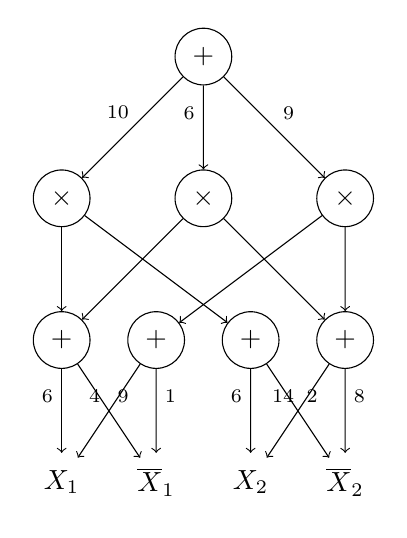
\begin{tikzpicture}
          [scale=.6,auto=left,every node/.style={draw, circle, inner sep = 0pt, minimum width = 0.72cm}]
        \node (n1) at (5,10) {$+$};
        \node (n2) at (2,7) {$\times$};
        \node (n3) at (5,7) {$\times$};
        \node (n4) at (8,7) {$\times$};
        \node (n5) at (2,4) {$+$};
        \node (n6) at (4,4) {$+$};
        \node (n7) at (6,4) {$+$};
        \node (n8) at (8,4) {$+$};
        \node[draw=none] (n9) at (2,1) {$X_1$};
        \node[draw=none] (n10) at (4,1) {$\overline{X}_1$};
        \node[draw=none] (n11) at (6,1) {$X_2$};
        \node[draw=none] (n12) at (8,1) {$\overline{X}_2$};

        \foreach \from/\to/\weight/\pos in {n1/n2/10/above left, n1/n3/6/above left, n1/n4/9/above right, n5/n9/6/above left, n5/n10/4/above left, n6/n9/9/above right, n6/n10/1/above right, n7/n11/6/above left, n7/n12/14/above left, n8/n11/2/above right, n8/n12/8/above right}
          \draw (\from) edge[->] node[\pos, draw=none, circle=none, minimum width=0.5cm, minimum height=0.2cm, inner sep=2pt]{\scriptsize \weight} (\to);

        \foreach \from/\to in {n2/n5, n2/n7, n3/n5, n3/n8, n4/n6, n4/n8}
          \draw (\from) edge[->] (\to);
      \end{tikzpicture}
    }

    (a)
  \end{minipage}\begin{minipage}{0.3333\textwidth}
    \centering
    \scalebox{0.7}{
      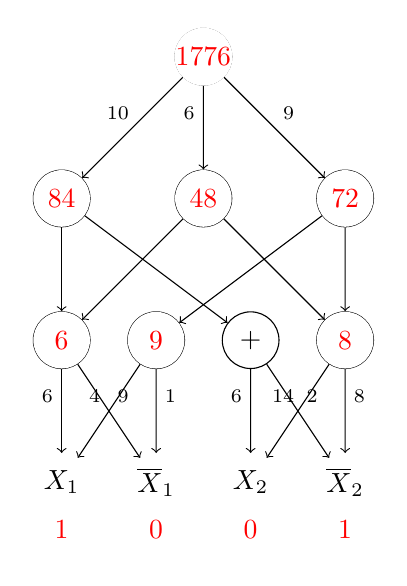
\begin{tikzpicture}
          [scale=.6,auto=left,every node/.style={draw, circle, inner sep = 0pt, minimum width = 0.72cm}]
        \node (n1) at (5,10) {$+$};
        \node (n2) at (2,7) {$\times$};
        \node (n3) at (5,7) {$\times$};
        \node (n4) at (8,7) {$\times$};
        \node (n5) at (2,4) {$+$};
        \node (n6) at (4,4) {$+$};
        \node (n7) at (6,4) {$+$};
        \node (n8) at (8,4) {$+$};
        \node[draw=none] (n9) at (2,1) {$X_1$};
        \node[draw=none] (n10) at (4,1) {$\overline{X}_1$};
        \node[draw=none] (n11) at (6,1) {$X_2$};
        \node[draw=none] (n12) at (8,1) {$\overline{X}_2$};

        \foreach \from/\to/\weight/\pos in {n1/n2/10/above left, n1/n3/6/above left, n1/n4/9/above right, n5/n9/6/above left, n5/n10/4/above left, n6/n9/9/above right, n6/n10/1/above right, n7/n11/6/above left, n7/n12/14/above left, n8/n11/2/above right, n8/n12/8/above right}
          \draw (\from) edge[->] node[\pos, draw=none, circle=none, minimum width=0.5cm, minimum height=0.2cm, inner sep=2pt]{\scriptsize \weight} (\to);

        \foreach \from/\to in {n2/n5, n2/n7, n3/n5, n3/n8, n4/n6, n4/n8}
          \draw (\from) edge[->] (\to);

        \node[draw=none, text=Red] (v1) at (2,0) {1};
        \node[draw=none, text=Red] (v1) at (4,0) {0};
        \node[draw=none, text=Red] (v1) at (6,0) {0};
        \node[draw=none, text=Red] (v1) at (8,0) {1};

        \node[draw=none, fill=white, text=Red] (s4) at (2,4) {6};
        \node[draw=none, fill=white, text=Red] (s4) at (4,4) {9};
        \node[draw=none, fill=white, text=Red] (s4) at (8,4) {8};
        \node[draw=none, fill=white, text=Red] (p7) at (2,7) {84};
        \node[draw=none, fill=white, text=Red] (p7) at (5,7) {48};
        \node[draw=none, fill=white, text=Red] (p7) at (8,7) {72};
        \node[draw=none, fill=white, text=Red] (s10) at (5,10) {1776};
      \end{tikzpicture}
    }

    (b)
  \end{minipage}\begin{minipage}{0.3333\textwidth}
    \centering
    \scalebox{0.7}{
      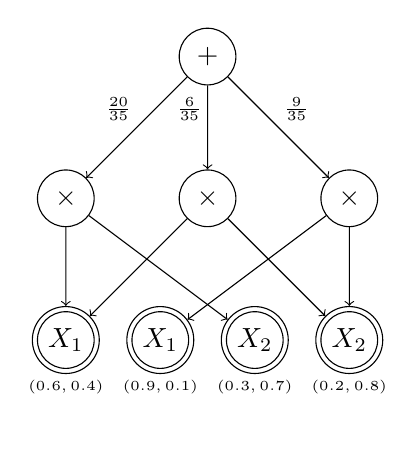
\begin{tikzpicture}
          [scale=.6,auto=left,every node/.style={draw, circle, inner sep = 0pt, minimum width = 0.72cm}]
        \node (n1) at (5,10) {$+$};
        \node (n2) at (2,7) {$\times$};
        \node (n3) at (5,7) {$\times$};
        \node (n4) at (8,7) {$\times$};
        \node (n5) at (2,4) {$X_1$};
        \node (n6) at (4,4) {$X_1$};
        \node (n7) at (6,4) {$X_2$};
        \node (n8) at (8,4) {$X_2$};

        \node[minimum width = 0.85cm] (n5) at (2,4) {};
        \node[minimum width = 0.85cm] (n6) at (4,4) {};
        \node[minimum width = 0.85cm] (n7) at (6,4) {};
        \node[minimum width = 0.85cm] (n8) at (8,4) {};

        \node[draw=none] (n9) at (2,3) {\tiny $(0.6, 0.4)$};
        \node[draw=none] (n10) at (4,3) {\tiny $(0.9, 0.1)$};
        \node[draw=none] (n11) at (6,3) {\tiny $(0.3, 0.7)$};
        \node[draw=none] (n12) at (8,3) {\tiny $(0.2, 0.8)$};

        \foreach \from/\to/\weight/\pos in {n1/n2/$\frac{20}{35}$/above left, n1/n3/$\frac{6}{35}$/above left, n1/n4/$\frac{9}{35}$/above right}
          \draw (\from) edge[->] node[\pos, draw=none, circle=none, minimum width=0.5cm, minimum height=0.2cm, inner sep=2pt]{\scriptsize \weight} (\to);

        \foreach \from/\to in {n2/n5, n2/n7, n3/n5, n3/n8, n4/n6, n4/n8}
          \draw (\from) edge[->] (\to);
      \end{tikzpicture}
    }

    (c)
  \end{minipage}

  \caption{
    \textbf{(a)} Uma rede soma-produto $\mathcal{S}$.
    \textbf{(b)} Exemplo de cálculo de $P(X_1, \overline X_2)$ (sem normalização) na rede soma-produto $\mathcal{S}$.
    \textbf{(c)} A rede soma-produto $\mathcal{S}$ convertida para a forma normal.
  }
  \label{fig:spn}
\end{figure}

\vspace{1em}

Numa rede soma-produto, definimos o \textbf{escopo} de um nó como o conjunto de variáveis presentes na sub-rede enraizada nele. Formalmente \cite{Zhao2015},

\begin{definition}[escopo]
  Seja $v$ é um nó. Se $v$ é uma folha indicando uma distribuição sobre uma variável $X$, então $\textrm{escopo}(v) = \{X\}$. Caso contrário, $\textrm{escopo}(v) = \cup_{w \in Ch(v)} \textrm{escopo}(w)$, onde $Ch(v)$ é o conjunto dos filhos de $v$ na rede soma-produto.
\end{definition}

A partir da definição de escopo, Poon e Domingos \cite{Poon2012} definem outras propriedades importantes sobre redes soma-produto:

\begin{definition}[SPN completa]
  Uma rede soma-produto é \textbf{completa} se cada nó do tipo soma tem filhos com o mesmo escopo.
\end{definition}

\begin{definition}[SPN consistente]
  Uma rede soma-produto é \textbf{consistente} se nenhuma variável aparece negada num filho de um nó produto e não-negada em outro.
\end{definition}

\begin{definition}[SPN decomponível]
  Uma rede soma-produto é \textbf{decomponível} se para todo nó produto $v$, a interseção dos seus filhos dois a dois é vazia, isso é, $\textrm{escopo}(v_i) \cap \textrm{escopo}(v_j) = \emptyset$ para todos $v_i, v_j \in Ch(v)$ com $i \neq j$.
\end{definition}

É fácil ver que se uma SPN é decomponível então ela é consistente.

\begin{definition}[SPN válida]
  Uma rede soma-produto é \textbf{válida} se ela define uma distribuição de probabilidade (não necessariamente normalizada).
\end{definition}

Poon e Domingos provaram \cite{Poon2012} que se uma rede soma-produto é completa e consistente, então ela é válida.

Com base nas propriedades acima, podemos agora definir uma rede soma-produto normal \cite{Zhao2015}:

\begin{definition}[forma normal]
  Uma SPN é dita \textbf{normal} se:

  \begin{enumerate}
    \item Ela é completa e decomponível.
    \item Os pesos das arestas saindo de cada nó da SPN são não-negativos e somam 1. Isso é, para todo nó soma $v$ com filhos $v_i \in Ch(v)$ e arestas com peso $w_i$ conectando $v$ e $v_i$, vale $w_i \geq 0$ e $\sum_{i=1}^{|Ch(v)|} w_i = 1$.
    \item Todo nó terminal da SPN é uma distribuição univariada sobre uma variável booleana e o tamanho do escopo de um nó soma é pelo menos 2 (nós soma cujo escopo é 1 são reduzidos em nós terminais).
  \end{enumerate}
\end{definition}

Zhao \emph{et al.} \cite{Zhao2015} provam que para toda SPN completa e consistente $\mathcal{S}$ existe uma SPN normal $\mathcal{S}'$ tal que $P_{\mathcal{S}}(\cdot) = P_{\mathcal{S}'}(\cdot)$ e $|\mathcal{S}'| = O(|\mathcal{S}|^2)$.

Um exemplo de uma SPN normal construída de uma SPN geral é mostrado na figura \ref{fig:spn} (c).

\section{Diagramas de decisão algébrica}

Diagramas de decisão algébrica (\emph{ADD}, do inglês \emph{Algebraic Decision Diagram}) são semelhantes a árvores de decisão, mas são mais compactos porque exploram subgrafos isomórficos. Formalmente são definidos como segue \cite{Bahar1993}:

\begin{definition}[diagrama de decisão algébrica]
  Um \textbf{diagrama de decisão algébrica} é uma representação num grafo acíclico dirigido enraizado de uma função real com entrada de variáveis booleanas: $f : \{0,1\}^N \rightarrow \mathbb{R}$. Há dois tipos de nós num ADD: nós terminais, cujo grau de saúda é 0, são associados com valores reais. Nós internos, cujo grau de saída é 2, são associados com variáveis booleanas $X_n$, $n \in [1, N]$.
\end{definition}

A figura \ref{fig:add} mostra uma árvore de decisão e uma ADD equivalente.

Zhao \emph{et al.} \cite{Zhao2015} estendem a definição original de diagrama de decisão algébrica permitindo que ele represente não apenas funções de variáveis booleanas, mas qualquer função de variáveis discretas com um domínio finito. Quando falamos em diagramas de decisão algébrica nesta monografia estamos nos referindo a essa extensão.

\begin{figure}
  \begin{minipage}{0.5\textwidth}
    \centering
    \scalebox{0.6}{
      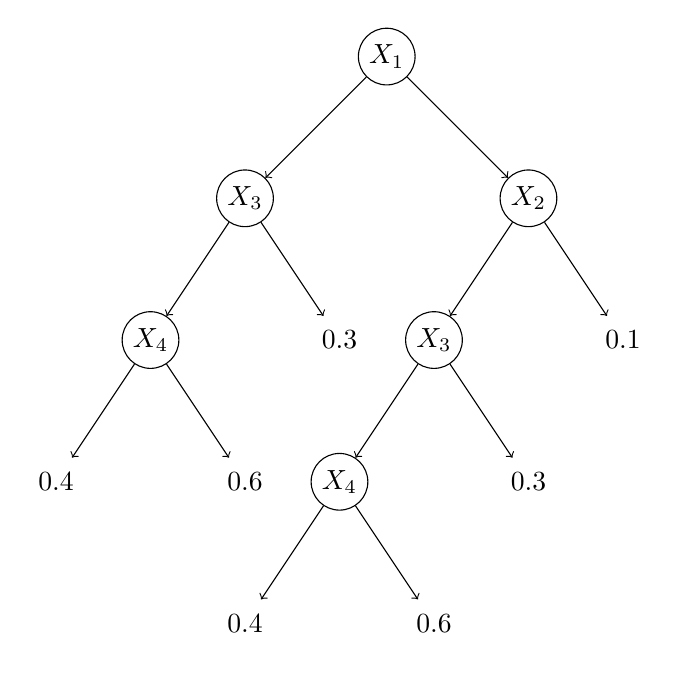
\begin{tikzpicture}
          [scale=.6,auto=left,every node/.style={draw, circle, inner sep = 0pt, minimum width = 0.72cm}]
        \node (x1) at (5,10) {$X_1$};
        \node (x31) at (2,7) {$X_3$};
        \node (x2) at (8,7) {$X_2$};
        \node (x41) at (0,4) {$X_4$};
        \node (x32) at (6,4) {$X_3$};
        \node (x42) at (4,1) {$X_4$};

        \node[draw=none] (a) at (-2,1) {0.4};
        \node[draw=none] (b) at (2,1) {0.6};
        \node[draw=none] (c) at (4,4) {0.3};
        \node[draw=none] (d) at (2,-2) {0.4};
        \node[draw=none] (e) at (6,-2) {0.6};
        \node[draw=none] (f) at (8,1) {0.3};
        \node[draw=none] (g) at (10,4) {0.1};

        \foreach \from/\to in {x1/x31, x1/x2, x31/x41, x31/c, x2/x32, x2/g, x41/a, x41/b, x42/d, x42/e, x32/x42, x32/f}
          \draw (\from) edge[->] (\to);
      \end{tikzpicture}
    }

    (a)
  \end{minipage}\begin{minipage}{0.5\textwidth}
    \centering
    \scalebox{0.6}{
      \begin{tikzpicture}
          [scale=.6,auto=left,every node/.style={draw, circle, inner sep = 0pt, minimum width = 0.72cm}]
        \node (x1) at (5,10) {$X_1$};
        \node (x31) at (2,7) {$X_3$};
        \node (x2) at (8,7) {$X_2$};
        \node (x41) at (0,4) {$X_4$};

        \node[draw=none] (a) at (-2,1) {0.4};
        \node[draw=none] (b) at (2,1) {0.6};
        \node[draw=none] (c) at (4,4) {0.3};
        \node[draw=none] (g) at (10,4) {0.1};

        \node[draw=none, text=white] (d) at (2,-2) {0.4};

        \foreach \from/\to in {x1/x31, x1/x2, x31/x41, x31/c, x2/x31, x2/g, x41/a, x41/b}
          \draw (\from) edge[->] (\to);
      \end{tikzpicture}
    }

    (b)
  \end{minipage}

  \caption{
    \textbf{(a)} Representação de uma função de variáveis binárias com árvore de decisão.
    \textbf{(b)} Representação da mesma função com diagrama de decisão algébrica.
  }
  \label{fig:add}
\end{figure}
